\chapter{Week 3: 2\textsuperscript{nd} - 8\textsuperscript{th} February }
\begin{itemize*}
	\item Find and remove bias on the sensors.
	\item Find the \gls{noisecomatrix} matrix used by the Kalman filter.
	\item Tune the Kalman Filter and compare it to the Complementary Filter. 
\end{itemize*}
	
	 \tocless\section{Sensor Bias}
	The bias on the sensors were found for the accelerometer by the means shown in figure \ref{Fig: Position to measure the bias} and they were found to be as follows:-
		\begin{equation}
		\begin{bmatrix}
		\gls{accbaisx}\\ \gls{accbaisy}\\\gls{accbaisz}
		\end{bmatrix} 
		=
		\begin{bmatrix}
		-2.223\\ 5.3447  \\9.17645
		\end{bmatrix}
		\end{equation}
		
		The bias on the gyroscope was found by placing the sensor on a flat surface and left to settle for five minutes so that the sensors would only measure there offsets and were found to be as follows:-
		
				\begin{equation}
				\begin{bmatrix}
				\gls{gyrobaisx}\\ \gls{gyrobaisy}\\\gls{gyrobaisz}
				\end{bmatrix} 
				=
				\begin{bmatrix}
				-34.163 \\ 20.156  \\-88.66
				\end{bmatrix}
				\end{equation}
	 \tocless\section{Measurement of the \gls{noisecomatrix} matrix}
ax It was possible to measure the \gls{noisecomatrix}  covariance matrix by obtaining various measurement from the sensors and estimating the noise present. The results were read to m-file and the covariance found using \textit{cov(x)} function in \textit{MatLab}. Hence the \gls{noisecomatrix}  matrix was calculated as follows:-
					\begin{equation}
			\gls{noisecomatrix}_a  = 		
                   \left[\begin{array}{ccc}
					\mathrm{cov(\gls{roll})}       &                 0                          & 0\\ 
					                                     0       & \mathrm{cov(\gls{pitch})}           & 0\\
					                                      0         &                0                          &\mathrm{cov(\gls{yaw})}
					\end{array} \right]
					\end{equation}
					Where \textit{cov(\gls{roll})} denotes the covariance of the \gls{roll} angle from the expected value.
	
Hence $\gls{noisecomatrix}_a$ was found as follows:-
						\begin{equation}
						\gls{noisecomatrix}_a  = 		
						1.0e-03\left[\begin{array}{ccc}
						0.2710      &                 0                          & 0\\ 
						0       & 0.1980           & 0\\
						0         &                0                          &NaN
						\end{array} \right]
						\end{equation}

By a similar manner one can find the $\gls{noisecomatrix}_g$ and define it as follows:-
	
							\begin{equation}
							\gls{noisecomatrix}_g  = 		
							1.0e-05\left[\begin{array}{ccc}
							0.1264      &                 0                          & 0\\ 
							0       & 0.2221           & 0\\
							0         &                0                          &0.0757
							\end{array} \right]
							\end{equation}
	
			 \tocless\section{Tuning of the Kalman Filter}
			Calculating the \gls{noisecoplantmatrix} matrix proved to be a much more difficult task. Very little real information regarding the noise present in the states was known. However, one method of tuning the filter is to leave on of the matrix fixed and scale the other as it is the ratio of \gls{noisecoplantmatrix} / \gls{noisecomatrix} which is important as seen in \cite{gordon_paper}. Hence, it was found that the ratio of the parameters affected the response and to a less degree the individual parameter values. Therefore \gls{noisecomatrix} was set to the theoretical value calculated and \gls{noisecoplantmatrix}  varied until an optimal response was achieved. The results of tuning the filter can be seen in figure {Fig: Kalman Filter Estimate and Complementary Filter Estimate }
	
		
\begin{figure}[h]
	\centering
	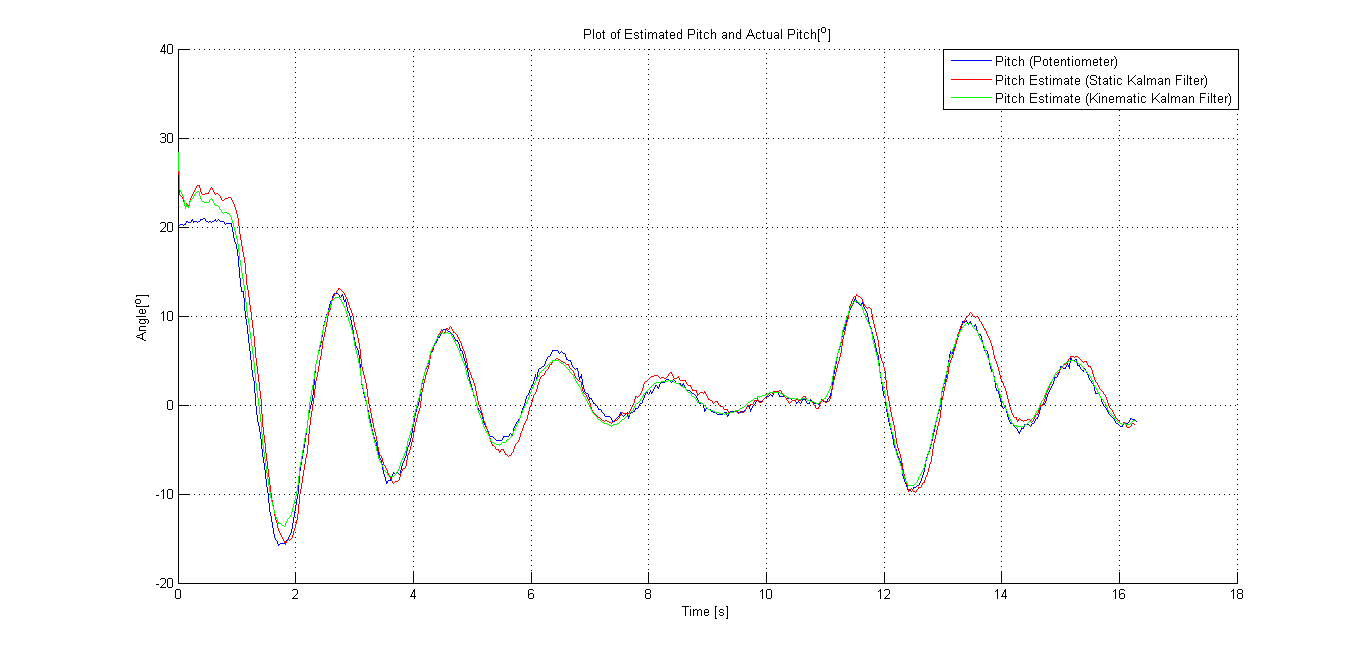
\includegraphics[width =0.6 \paperwidth, height = 7cm]{\DocRoot/images/kalman_comp}
	\caption{Plot of Kalman Filter Estimate, Complementary Filter Estimate and Actual Angle of the device}
	\label{Fig: Kalman Filter Estimate and Complementary Filter Estimate }
\end{figure}

For the above graph $K_{p\gls{pitch}}$ and $K_{i\gls{pitch}}$ are equal to 3.5902 and 2.0522 respectively. While \gls{kalmangain} was found to be as follows:-

							\begin{equation}
							\gls{kalmangain}_{\gls{pitch}}  = 		
							\left[\begin{array}{cc}
							0.032064         &      0.0001017                         \\ 
							0.0085871       &     0.996498           
							\end{array} \right]
							\end{equation}


	 \tocless\section{Chart Depicting how the Kalman Filter Works}
		\begin{center}
			\begin{tikzpicture}[scale=0.65, transform shape]
			
			%
			% Styles for states, and state edges
			%
			\tikzstyle{state} = [{rectangle, rounded corners, draw=black, very thick, text width=20.0em, minimum height=4em, text centered}]
			\tikzstyle{stateEdgePortion} = [black,thick];
			\tikzstyle{stateEdge} = [stateEdgePortion,->];
			\tikzstyle{edgeLabel} = [pos=0.5, text centered, font={\sffamily\small}];
			
			
			%
			% Position States
			%
			\node[state, name=predict] {{{\LARGE}{\bf Model Update} (\enquote{Predict})}   \\ 
				{   (1) Predict State  \\  \vspace{-0.25cm}
					\hh $\hat{x}^{*}_{k} = \gls{Transitionmatrix}\hat{x}_{k-1} + \gls{Bmatrix}u_{k}$\\ 
					(2) Predict Error Covariance \\ \vspace{-0.25cm}
					\hh $\gls{covariancematrix}^* = \gls{Transitionmatrix}\gls{covariancematrix}_{-1}\gls{Transitionmatrix}^{\intercal} + \gls{noisecoplantmatrix}$}};
			
			
			\node[state, name=correct, right of=predict, xshift=20em] {{\bf Measurement Update} (\enquote{Correct}) \\ 
				{   (1) Compute Kalman Gain\\  \vspace{-0.25cm}
					\hh $\gls{kalmangain}_{k} = \gls{covariancematrix}^*\gls{Cmatrix}^{\intercal}(\gls{Cmatrix}\gls{covariancematrix}^*\gls{Cmatrix}^{\intercal} + \gls{noisecomatrix})^{-1}$\\ 
					(2) Update Estimate with Measurement $\gls{measurement}$ \\ \vspace{-0.25cm}
					\hh $\hat{x}_k = \hat{x}^{*}_k + \gls{kalmangain}_k(z_k - \gls{Cmatrix}\hat{x}_k^{*})$\\
					(3) Update Error Covariance  \\ \vspace{-0.25cm}
					\hh $\gls{covariancematrix} = (I - \gls{kalmangain}_k\gls{Cmatrix})\gls{covariancematrix}^{*}$
					
				}};
				
				
				%
				% Connect States via edges
				%
				\draw (predict.north) 
				edge[stateEdge, bend left=45] node[edgeLabel, xshift=-3em]{} 
				(correct.north); 
				
				\draw ($(predict.west) + (0,2.5em)$) 
				edge[stateEdgePortion] node[edgeLabel, yshift=+2.1cm]{} 
				($(predict.east) + (0,2.5em)$); 
				
				\draw (correct.south) 
				edge[stateEdge, bend left=45] node[edgeLabel, xshift=-3em]{} 
				(predict.south); 
				
				\draw ($(correct.west) + (0,4.0em)$) 
				edge[stateEdgePortion] node[edgeLabel, yshift=+2.1cm]{} 
				($(correct.east) + (0,4.0em)$); 
				
				
				
				% 
				% inital states to start the filter
				%
				\node[ name=inital, below of=predict, left of=predict, xshift = -3em ,yshift=-8em]{Initial Estimates for $\hat{x}_{k-1}$ and $\gls{covariancematrix}_{-1}$};
				
				\draw ($(inital.north) + (0,0)$) 
				edge[stateEdge] node[edgeLabel, yshift=+2.1cm]{} 
				($(predict.south) + (-5.4em,0)$); 
				\end{tikzpicture}
			\end{center}
